\usepackage{etex} %эта магическая херь избавляет от переполнения регистров TeX а!!!

\mode<article>{\usepackage{fullpage}}
\mode<presentation>{
    \usetheme{Madrid}
    \useoutertheme{shadow}
} 

\usepackage[utf8]{inputenc}
\usepackage[russian]{babel}
\usepackage{indentfirst}
\usepackage{graphicx}

\usepackage{amsmath}
\usepackage{amsfonts}
\usepackage{amsthm}
%\usepackage{algorithm}
%\usepackage{algorithmic}

%\usepackage[all]{xy}

\date{Лекция по дисциплине <<методы и средства защиты компьютерной информации>> (\today)}
\author[М.~М.~Шихов]{Михаил Шихов \\ \texttt{\underline{m.m.shihov@gmail.com}}}

%%для рисования графов пакетом xy-pic
%\entrymodifiers={++[o][F-]}

%%для псевдокода алгоритмов (algorithm,algorithmic)
%\renewcommand{\algorithmicrequire}{\textbf{Вход:}}
%\renewcommand{\algorithmicensure}{\textbf{Выход:}}
%\renewcommand{\algorithmiccomment}[1]{// #1}
%\floatname{algorithm}{Псевдокод}

%\setbeamercolor{alerted text}{fg=-green} %gyan, blue, green, -green


\title[Ретро-криптоанализ]{Ретро-криптоанализ. Дополнительные задания по дисциплине <<методы и средства защиты компьютерной информации>>}

\begin{document}


%титул и содержание статьи
\mode<article>{\maketitle\tableofcontents}

%титул и содержание презентации
\frame<presentation>{\titlepage}
\begin{frame}<presentation>[allowframebreaks]
    \frametitle{Содержание}
    \tableofcontents
\end{frame}

\begin{frame}
    \begin{figure}
        \begin{center}
            \mode<presentation>{ 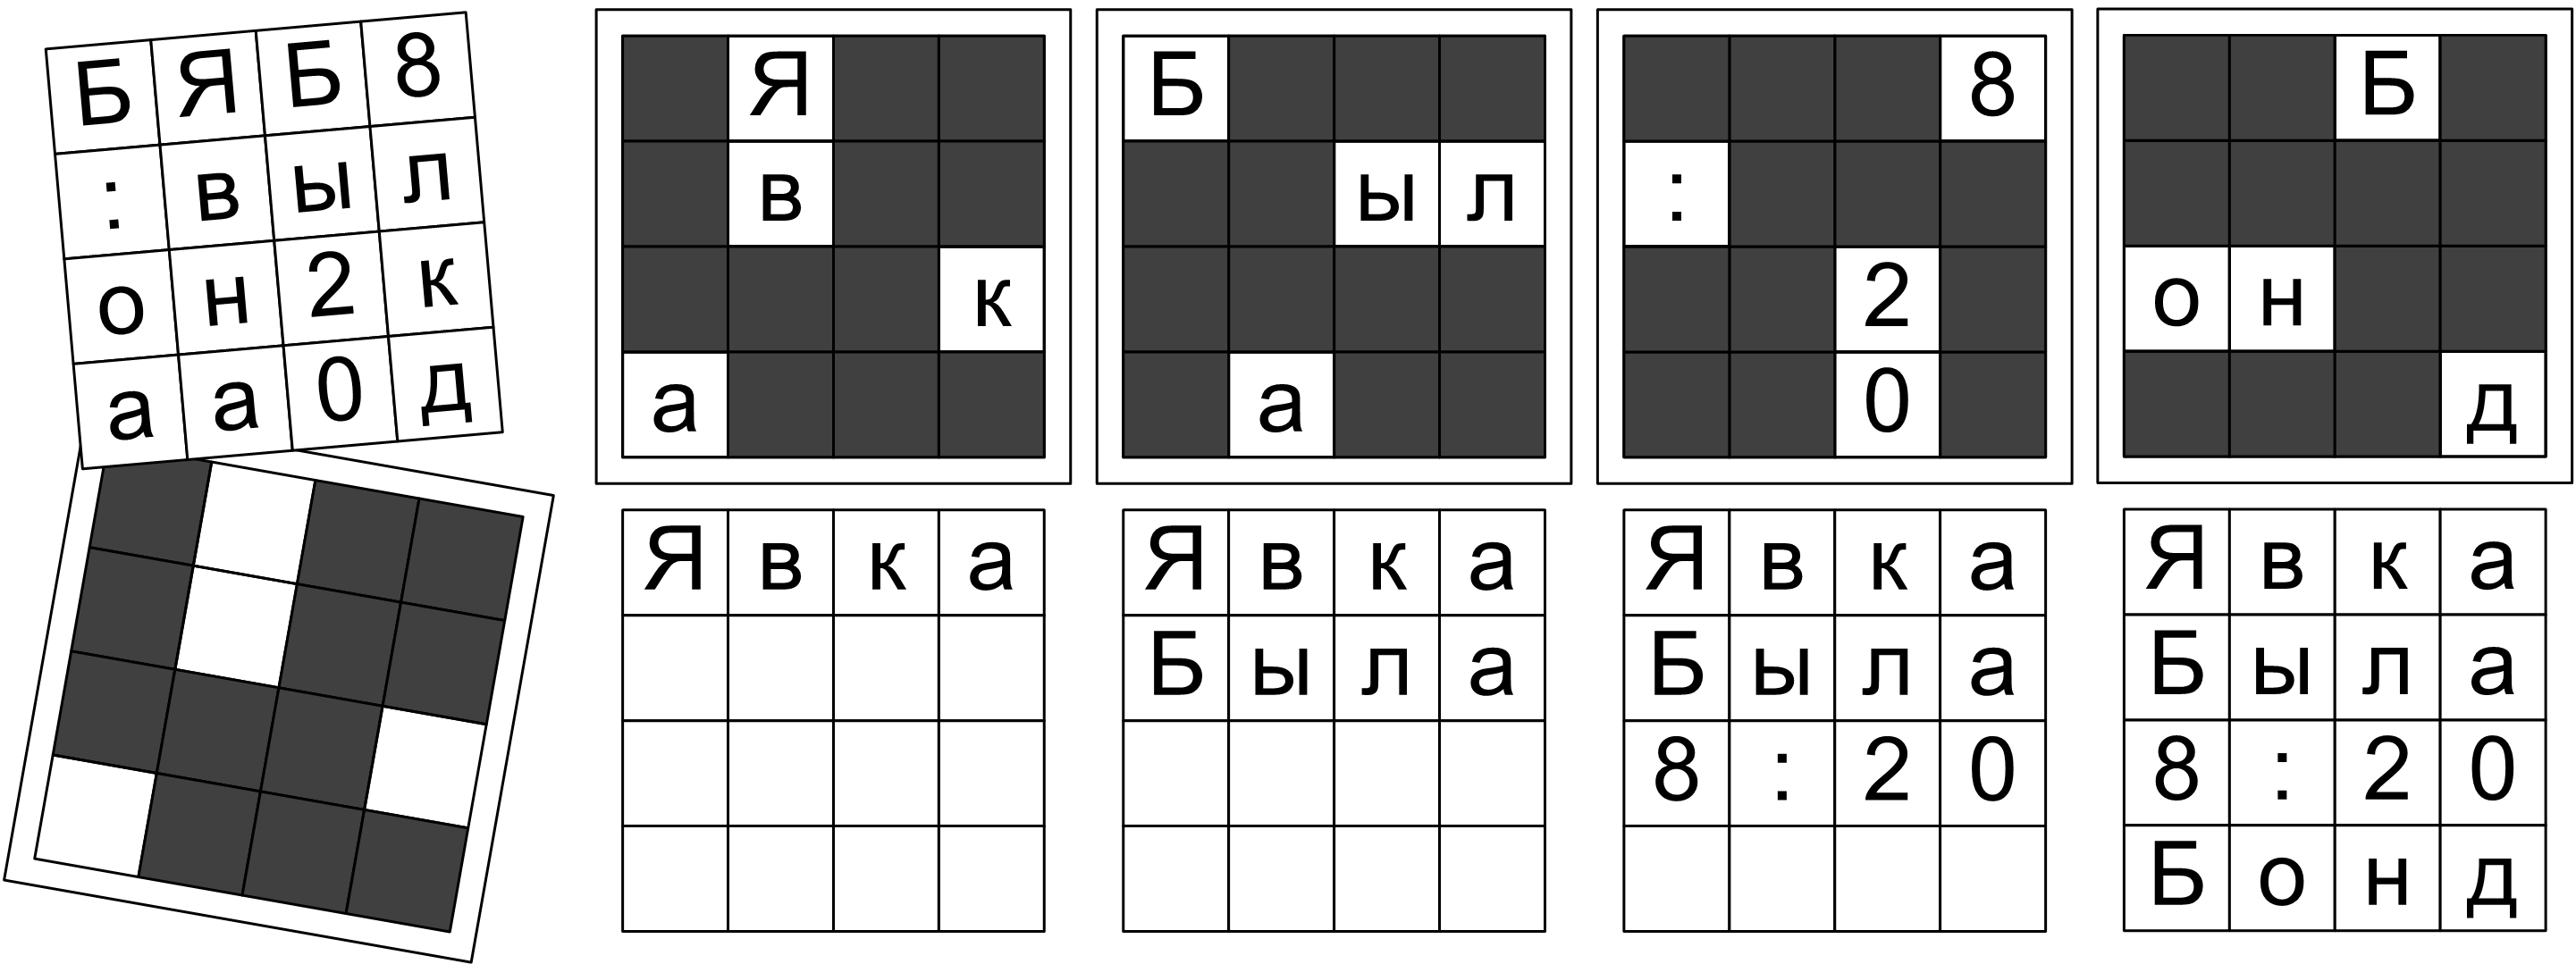
\includegraphics[width=.99\textwidth]{pict/rotation2} }
            \mode<article>{ 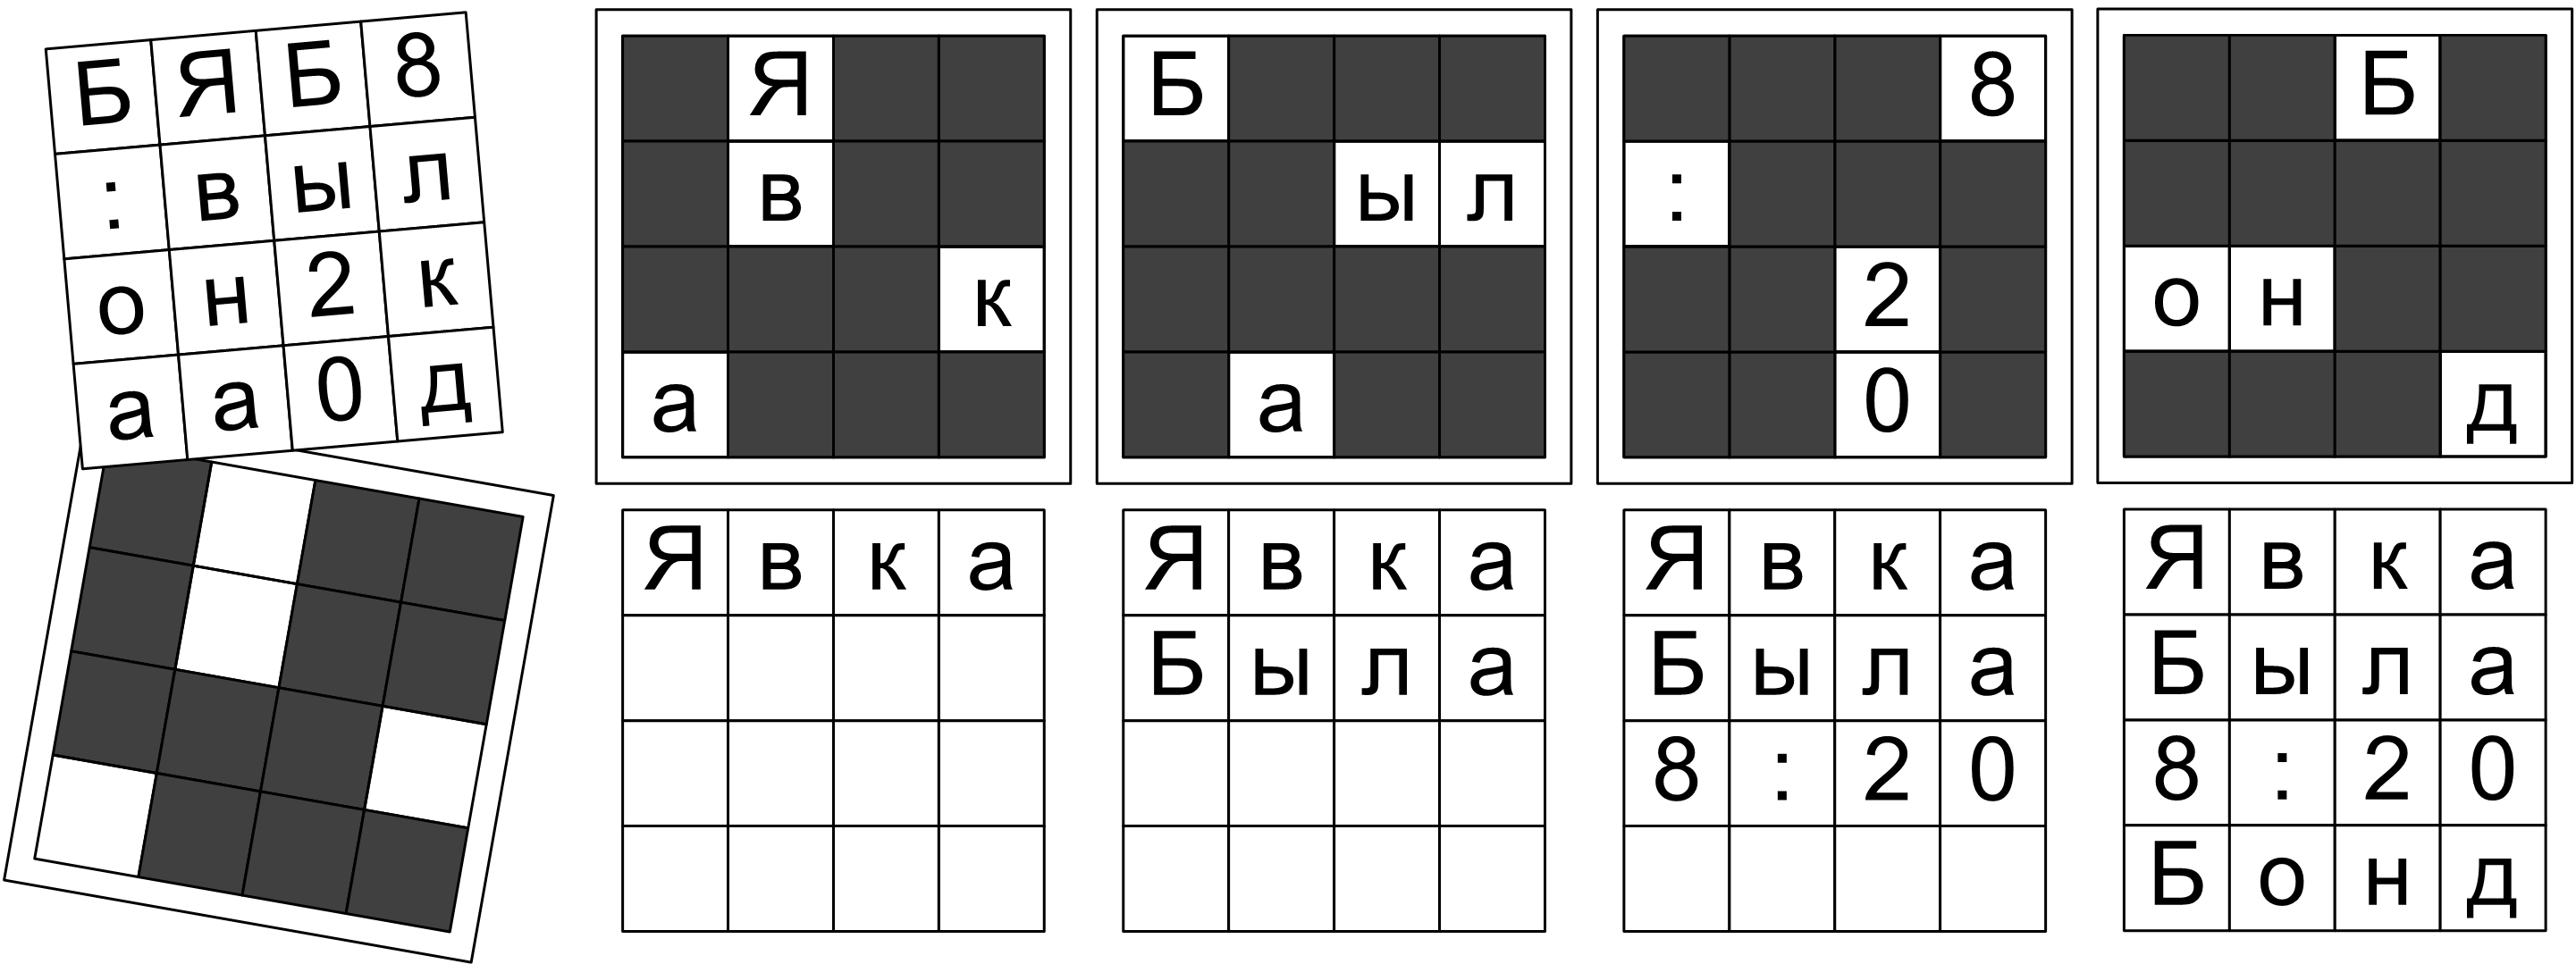
\includegraphics[width=.9\textwidth]{pict/rotation2} } 
        \end{center}
    \end{figure} 
    \mode<article>{см. рис. \ref{pict:rotation2}}
\end{frame}


\section{Теория}


\subsection{Вращения}


\begin{frame}
    \frametitle{Решетка}
    \framesubtitle{Вращения}
    \begin{figure}
        \begin{center}
            \mode<presentation>{ 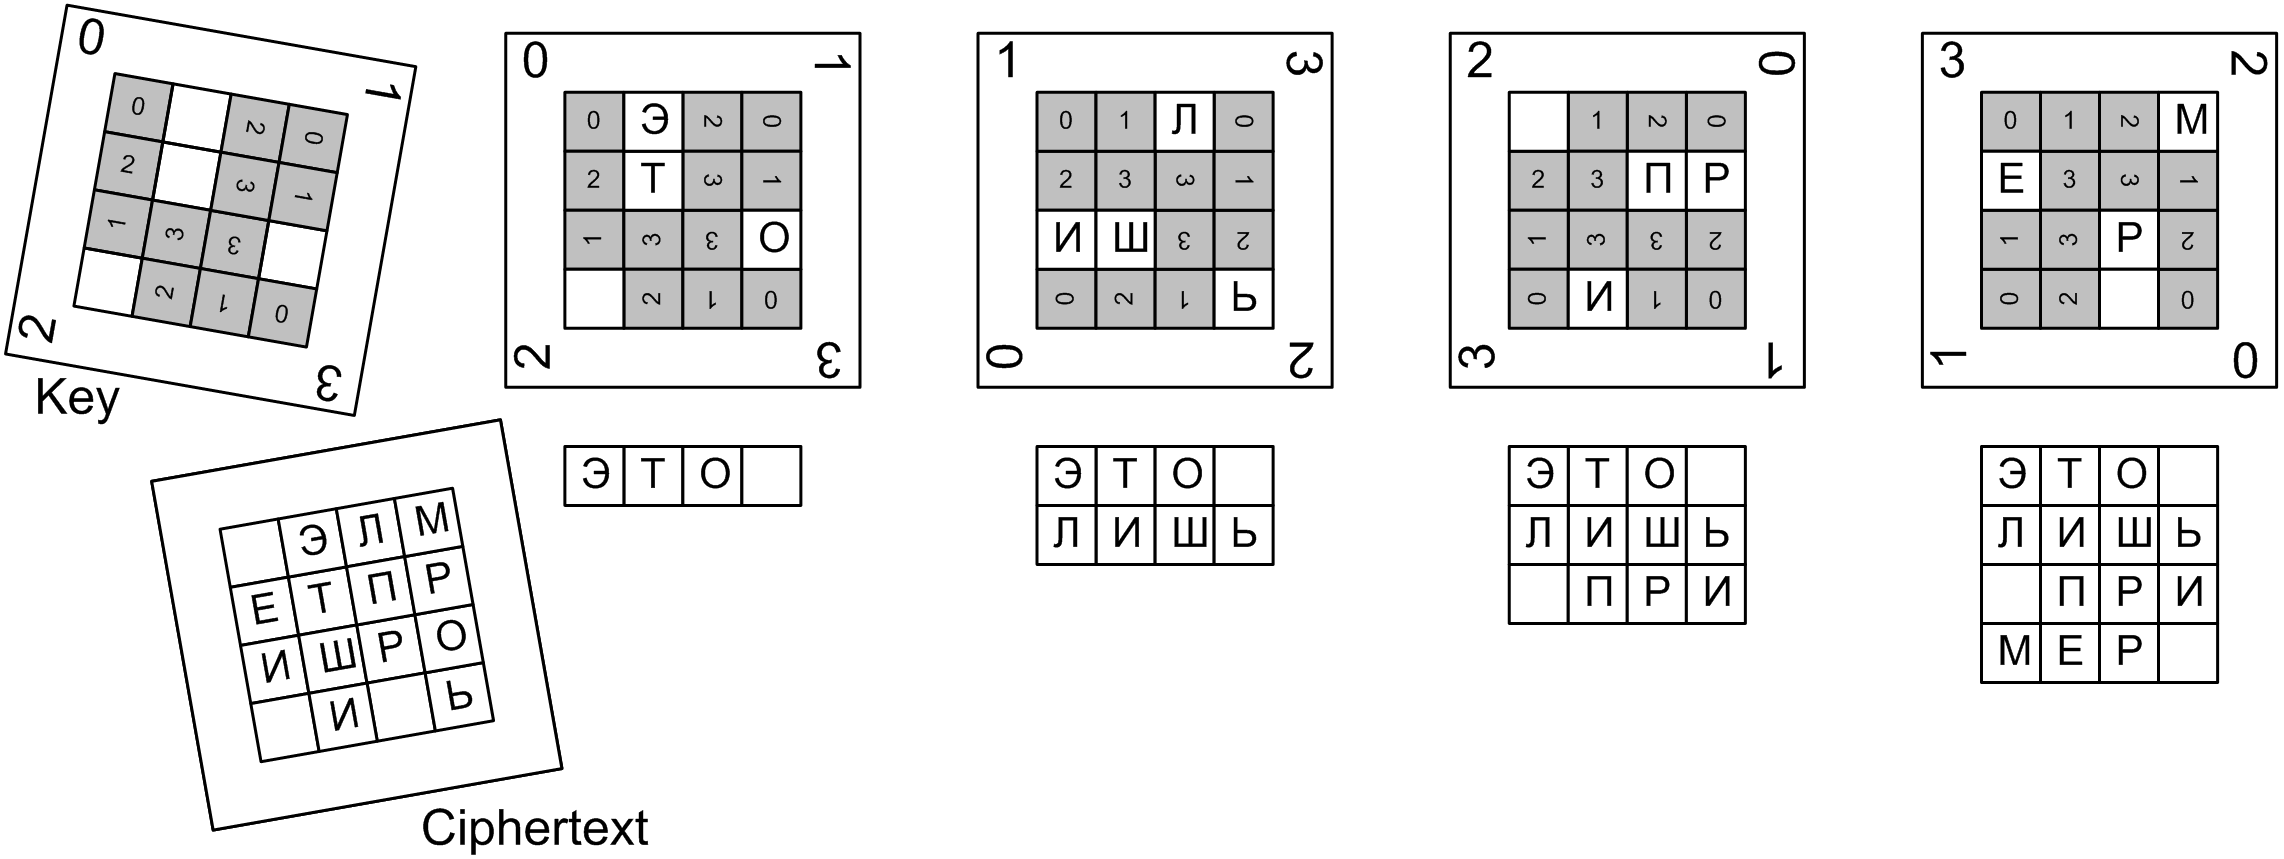
\includegraphics[width=.99\textwidth]{pict/rotation} }
            \mode<article>{ 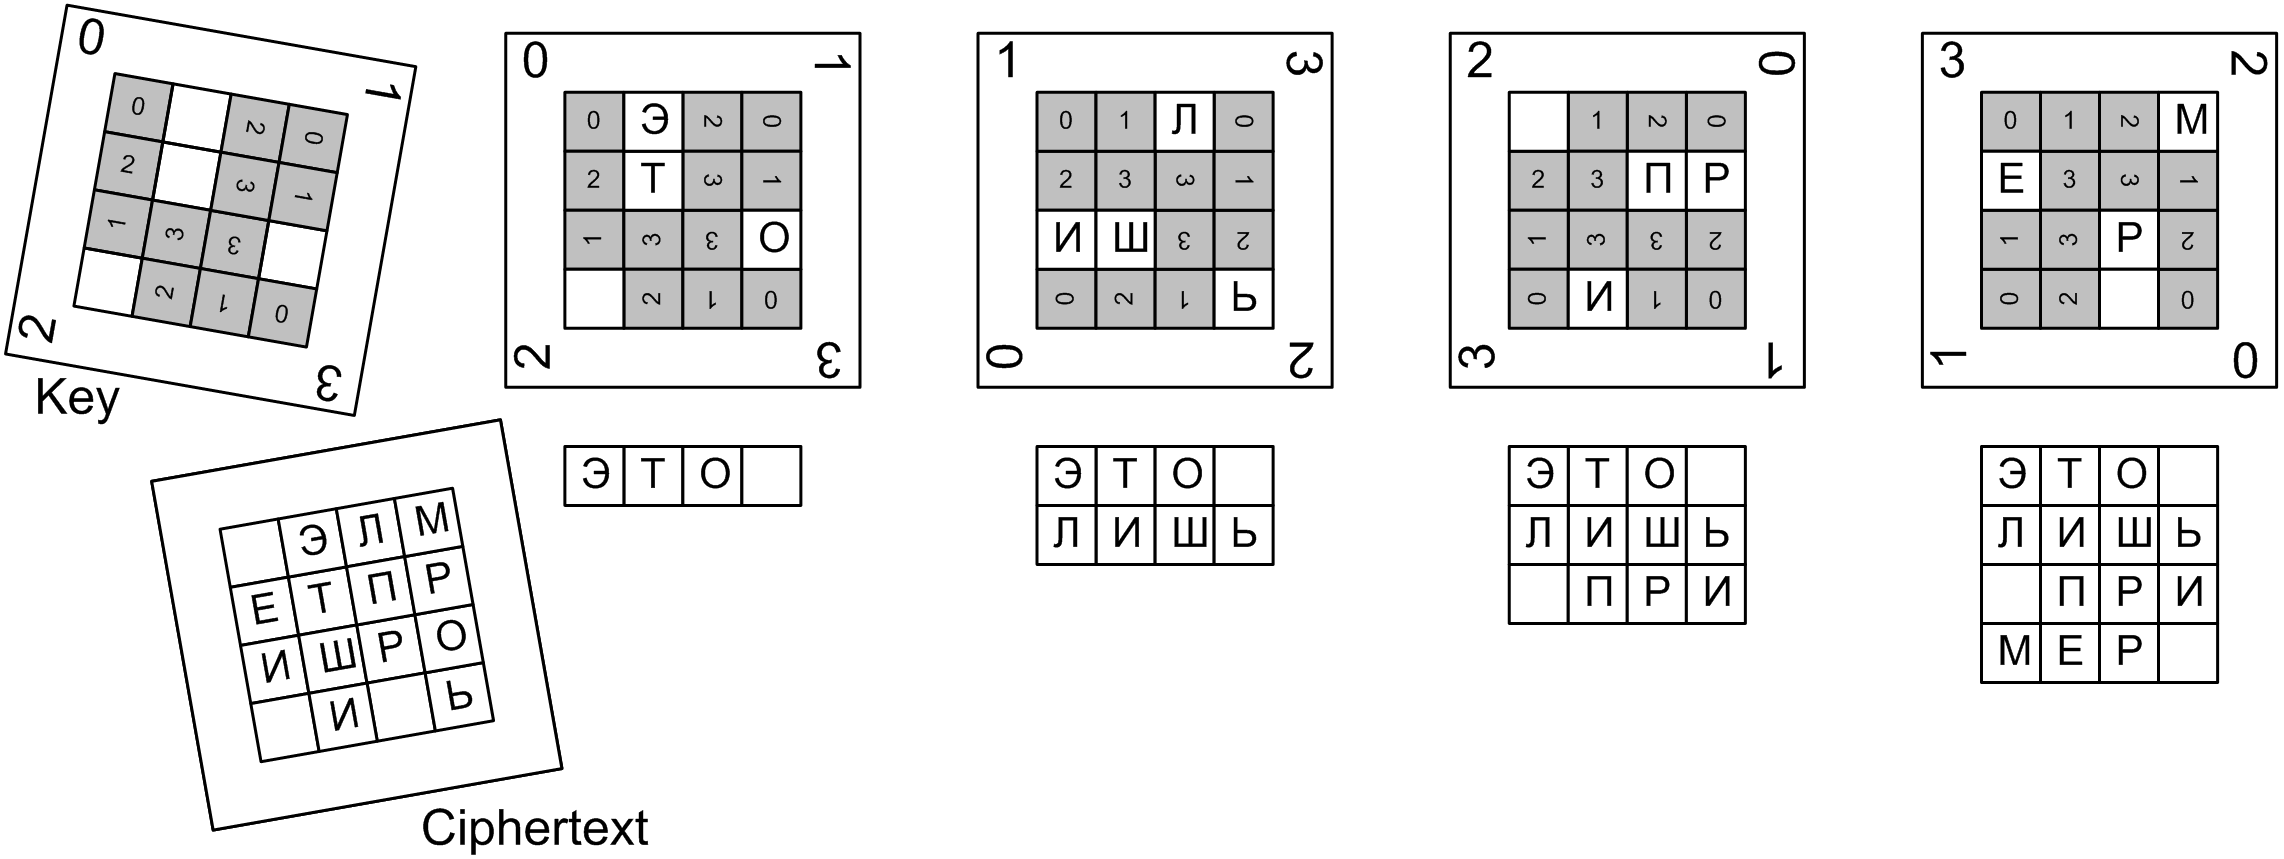
\includegraphics[width=.9\textwidth]{pict/rotation} } 
            \caption{Вращения}\label{pict:rotation}
        \end{center}
    \end{figure} 
    \mode<article>{см. рис. \ref{pict:rotation}}
\end{frame}


\subsection{Отражения в 2D}


\begin{frame}
    \frametitle{Решетка}
    \framesubtitle{Отражения в 2D}
    \begin{figure}
        \begin{center}
            \mode<presentation>{ 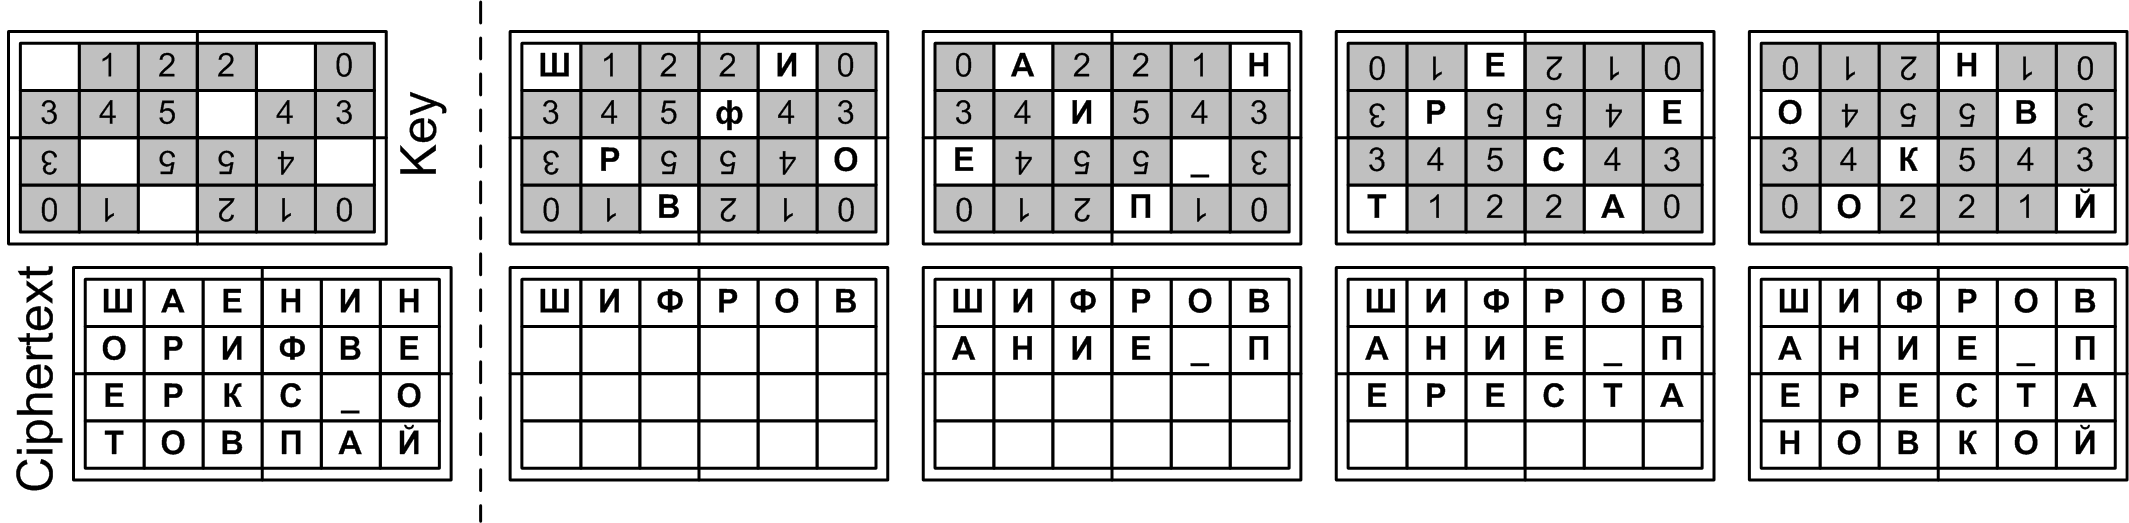
\includegraphics[width=.99\textwidth]{pict/flip} }
            \mode<article>{ 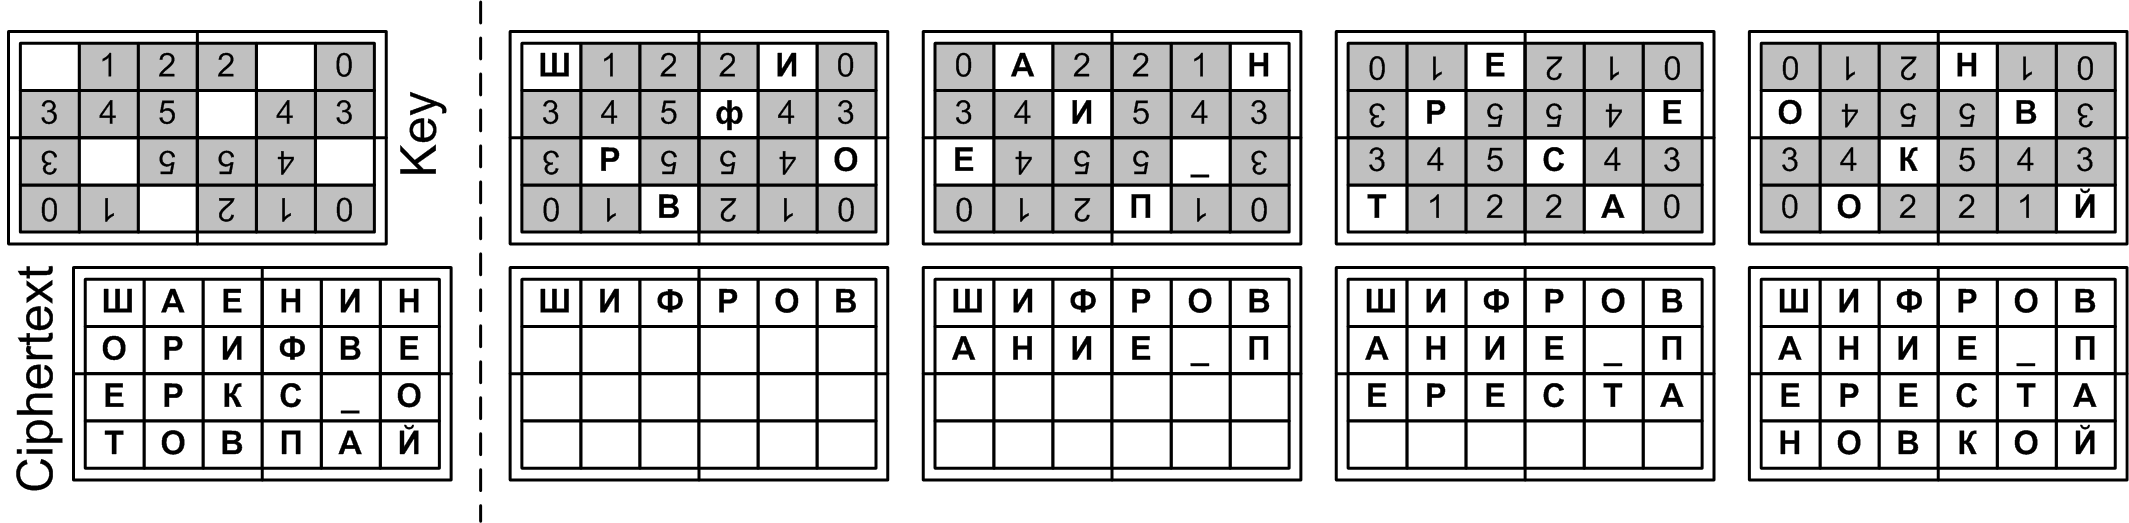
\includegraphics[width=.9\textwidth]{pict/flip} } 
            \caption{Отражения 2D}\label{pict:flip}
        \end{center}
    \end{figure} 
    \mode<article>{см. рис. \ref{pict:flip}}
\end{frame}


\subsection{Отражения в 3D}


\begin{frame}
    \frametitle{Решетка}
    \framesubtitle{Отражения в 3D}
    
    Отражения легко распространяются на $N$-мерное пространство.
    \begin{figure}
        \begin{center}
            \mode<presentation>{ 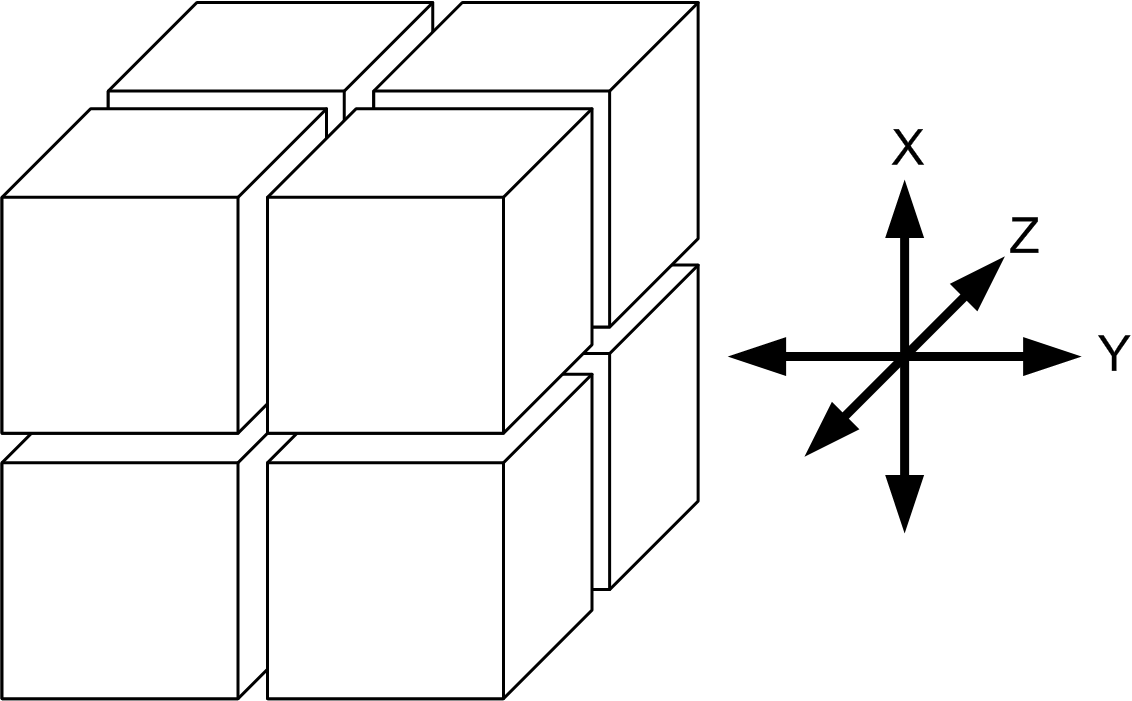
\includegraphics[width=.60\textwidth]{pict/flip3d} }
            \mode<article>{ 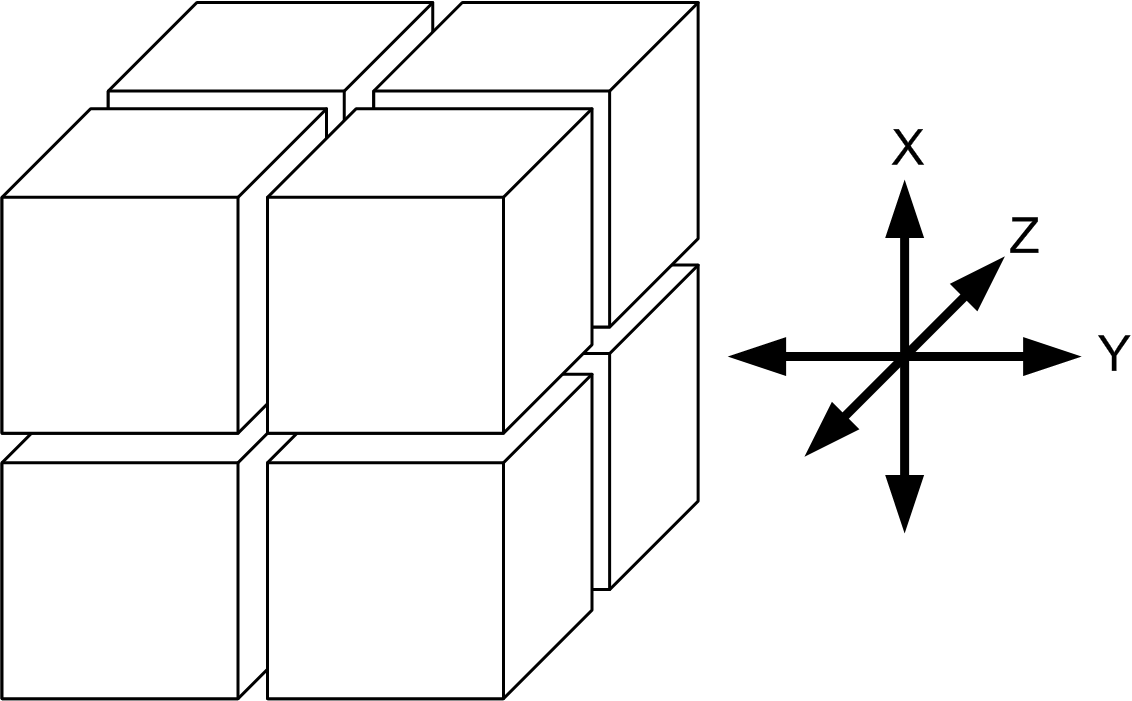
\includegraphics[width=.6\textwidth]{pict/flip3d} } 
            \caption{Отражения в 3D}\label{pict:flip3d}
        \end{center}
    \end{figure} 
    \mode<article>{см. рис. \ref{pict:flip3d}}
\end{frame}


\section{Задания. Перестановочные шифры.}


\subsection{Вращения}

\begin{frame}[fragile]
    \frametitle{Решетка. Вращения}
    \framesubtitle{Пояснения}
        
    На следующих двух слайдах приведены два шифротекста, полученных с помощью одного и того же ключа. Криптоаналатик знает начало открытого текста, соответствующего первому шифротексту\ldots
    
    Расшифруйте оба шифротекста\footnote{Каждый следующий поворот решетки может быть на 90, 180, 270 гдадусов}.
\end{frame}


\begin{frame}[fragile]
    \frametitle{Решетка}
    \framesubtitle{Вращения. Утечка открытого текста (начало фразы)}
    
    \begin{table}[ht]
        \centering
        \begin{tabular}[c]{|l@{}|l@{}|l@{}|l@{}|l@{}|l@{}|l@{}|l@{}|l@{}|l@{}|l@{}|l@{}|}
            \hline
            Х&С&З&К&Ц&О&Р&Л&А&О&З&О\\ \hline 
            И&И& &П&К&О&М&Е&Ш&В& &И\\ \hline 
            О&А&Й& &Т&О&Л& &В& &О&Р\\ \hline 
            Н&Л&Ы&К&К&М& &В&О&П&Е&Р\\ \hline 
            И&С& &О&И&З&П&М&Е& &Р&К\\ \hline 
            О& &Х&Л&И&Р&З&О&Л&Я&Т&Н\\ \hline 
            А&Ы&Й& &А&П&К&Х&,&И&З&Р\\ \hline 
            О&В&Т&Е&Д&Е&Г&О&Д&К&Р&Е\\ \hline 
            Н&О&И&К&О&Й& &Л&Е&А& &Т\\ \hline 
            А&А& &У&Е&В&К&И&Т&М&О&Е\\ \hline 
             &Н& &П&Т&Л&Б&И&Ы&Л& &В\\ \hline 
            К&Ф&Е&И& &С&Н& &К&В&А&И\\ \hline 
        \end{tabular}
    \end{table}
\begin{verbatim}
ХОРОШИЙ ПРИМЕР ХАКЕРКОЙ АТАКИ Б
\end{verbatim}
\end{frame}


\begin{frame}[fragile]
    \frametitle{Решетка}
    \framesubtitle{Вращения. Перехват после утечки}
    
    \begin{table}[ht]
        \centering
        \begin{tabular}[c]{|l@{}|l@{}|l@{}|l@{}|l@{}|l@{}|l@{}|l@{}|l@{}|l@{}|l@{}|l@{}|}
            \hline
            К&Р&С&И&К&О&З&Л&Т&Л&Е&А\\ \hline 
            А& &П&О&С& &;&Я&Я&К&!&Т\\ \hline 
            В&Б&У&А&О&П&Е&Ш&Ш&Ж&А&Ы\\ \hline 
            Т& &Е&И&М&Ч&К&У&,&К&А&И\\ \hline 
            ,&И&Т&Т&Ь& &З&Р&Е& &Б&П\\ \hline 
            Р&Я&Т&М&О& &И&К&Ш&Л&А&Л\\ \hline 
            -&О&К&О&У& &Ш&М&О&О&П&П\\ \hline 
            О&Ы& &Т&Е&К&Л&В&О&Ы&И&Ч\\ \hline 
            К&М&А&!&О&Т&О&Е&К&П&Ч&Р\\ \hline 
            И&К&А&У&.& &Т&Е&,&К&П&И\\ \hline 
            У&З&С&Д& &Р&Я&В&,&О&Т&В\\ \hline 
            И&Ы&А&М&Н&?&?&О&Е&Е&Ч&?\\ \hline 
        \end{tabular}
    \end{table}
    Ключ использовался тот же, что и на предыдущем слайде.
\end{frame}


\subsection{Отражения в 2D}


\begin{frame}[fragile]
    \frametitle{Решетка. Отражения в 2D}
    \framesubtitle{Пояснения}
        
    На следующих двух слайдах приведены два шифротекста, полученных с помощью одного и того же ключа. Криптоаналатик знает начало открытого текста, соответствующего первому шифротексту\ldots
    
    Расшифруйте оба шифротекста.
\end{frame}


\begin{frame}[fragile]
    \frametitle{Решетка}
    \framesubtitle{Отражения в 2D. Утечка открытого текста (начало фразы)}
    
    \begin{table}[ht]
        \centering
        \begin{tabular}[c]{|l@{}|l@{}|l@{}|l@{}|l@{}|l@{}|l@{}|l@{}|l@{}|l@{}|l@{}|l@{}|l@{}|l@{}|l@{}|l@{}|l@{}|l@{}|}
            \hline
            Д&С&О& &В&Т&Е&С&З&О&И& &Т&Н&А& &И&С\\ \hline 
            Л&А&Я& &Е&М& &А&А&Р&С&Н&Е&Б&Ш&И&Ф&Р\\ \hline 
            Я& &О&П&Т&И&Е&Р&Р&В&Ч&А&И& &Е&И&С&К\\ \hline 
            О&Н&Х&Н& &А&М&Ф&Р& &А&У&У&,&Р&Р&В&Ш\\ \hline 
             &Е&О&А&Н&Г&К&И&М&О&В&Е&Т&Н&О&И&Е&Н\\ \hline 
            Т& & &П&Р&О& &Р&Д&Ц&М&Е&О&И& &О&О&П\\ \hline 
            С&Т&У&П&И&С&З&А&Л&А&В&Н&Е&Д&О&С&Т&Н\\ \hline 
            Е&О&Н&И&Я&,& &Н&О&.&К&А&И&К& &Н&К&А\\ \hline 
        \end{tabular}
    \end{table}
\begin{verbatim}
ЗАШИФРОВАН ФРАГМЕНТ ПРОИЗВЕДЕНИЯ
\end{verbatim}
\end{frame}


\begin{frame}[fragile]
    \frametitle{Решетка}
    \framesubtitle{Отражения в 2D. Перехват после утечки}
    
    \begin{table}[ht]
        \centering
        \begin{tabular}[c]{|l@{}|l@{}|l@{}|l@{}|l@{}|l@{}|l@{}|l@{}|l@{}|l@{}|l@{}|l@{}|l@{}|l@{}|l@{}|l@{}|l@{}|l@{}|}
            \hline
            Н&С&Ц&Е& &О&К&О&К& &З&Н&Н&А&Н&И&Ц&Я\\ \hline 
            К&Л&Е&В& &И&О& &А&Е&В&П& &К&Ж&Д&Ы&Й\\ \hline 
            Л&Е& &В&Р&О&Т&Е&У&С&Б&О&Т&А&Н& &Ы&М\\ \hline 
             &В&Н& &Е&Я&К&Т&В&А&Е&Л&М& &Н& &Е&Я\\ \hline 
            С&Е&Е&Н&Т&Е&Т&С& &Ь&М&О& & &И&Я&С&Б\\ \hline 
            Р&А& &Щ&С&Т&И&А&Л&М&И&Е&Т&Ь&Н&Ы&Н&Ы\\ \hline 
            .&Ч&Е&Г&Й& & &С&Р&О&В&О&Н&И&И&Л&О&М\\ \hline 
            М&В&А&Н&И&Е&Я& & &?&Т&.&Н&В& &К&А&О\\ \hline 
        \end{tabular}
    \end{table}
    Ключ использовался тот же, что и на предыдущем слайде.
\end{frame}


\subsection{Отражения в 3D}

\begin{frame}[fragile]
    \frametitle{Решетка. Отражения в 3D}
    \framesubtitle{Пояснения}
        
    На следующих восьми слайдах приведены два шифротекста, полученных с помощью одного и того же ключа. Криптоаналатик знает начало открытого текста, соответствующего первому шифротексту\ldots
    
    Размерность шифра $4\times 6\times 6$.
    
    Расшифруйте оба шифротекста\footnote{Приводятся <<срезы>> шифра (0-й,1-й,2-й,3-й). При шифровании <<срезы>> заполняются последовательно: сначала 0-й, затем 1-й и т.д. Затем следует отражение относительно одной из трех плоскостей и заполнение повторяется}.
\end{frame}


\begin{frame}[fragile]
    \frametitle{Решетка}
    \framesubtitle{Отражения в 3D. Утечка открытого текста (начало фразы)}
    
    \begin{table}[ht]
        \caption{0-й срез}
        \centering
        \begin{tabular}[c]{|l|l|l|l|l|l|}
            \hline
            В&Е&,&К&И&А\\ \hline
            З&К&Н&А& &З\\ \hline
            Л&А&Н&Е&Н&А\\ \hline
            А&И&Ч&Н&Т&Н\\ \hline
            В&Т&А&Е&А& \\ \hline
            О& &П&М&Е&О\\ \hline
        \end{tabular}
    \end{table}
\begin{verbatim}
В ЗАМЕЧАТЕЛЬНОЙ СК
\end{verbatim}
\end{frame}


\begin{frame}[fragile]
    \frametitle{Решетка}
    \framesubtitle{Отражения в 3D. Утечка открытого текста (начало фразы)}
    
    \begin{table}[ht]
        \caption{1-й срез}
        \centering
        \begin{tabular}[c]{|l|l|l|l|l|l|}
            \hline
            Л& &Ч&О&Р& \\ \hline
            А&О&Ц&О&И&Я\\ \hline
            А&Э&М&Р&А& \\ \hline
            Т&П&Т&Е&Е&А\\ \hline
            С& &Л& &Р&Р\\ \hline
            Т&Ь& &Р&А&У\\ \hline
        \end{tabular}
    \end{table}
\end{frame}


\begin{frame}[fragile]
    \frametitle{Решетка}
    \framesubtitle{Отражения в 3D. Утечка открытого текста (начало фразы)}
    
    \begin{table}[ht]
        \caption{2-й срез}
        \centering
        \begin{tabular}[c]{|l|l|l|l|l|l|}
            \hline
            .&Ю&К&С&И&Н\\ \hline
            С&Е&Щ& &С&О\\ \hline
            Е&В&С&Г&И&О\\ \hline
            Й&О&Я& &О&З\\ \hline
            Д&.&П&И&Й&А\\ \hline
            С&Р& &Б&,&Л\\ \hline
        \end{tabular}
    \end{table}
\end{frame}


\begin{frame}[fragile]
    \frametitle{Решетка}
    \framesubtitle{Отражения в 3D. Утечка открытого текста (начало фразы)}
    
    \begin{table}[ht]
        \caption{3-й срез}
        \centering
        \begin{tabular}[c]{|l|l|l|l|l|l|}
            \hline
            И&Щ&Е&А&У&Н\\ \hline
            Е& &Т&Н&М&Е\\ \hline
             &П&У&С&К&Ш\\ \hline
            Т&Т&А&А&Н&В\\ \hline
            И&Й&Р&Г&Е&Н\\ \hline
            Т&А&Р& &К&.\\ \hline
        \end{tabular}
    \end{table}
\end{frame}


\begin{frame}[fragile]
    \frametitle{Решетка}
    \framesubtitle{Отражения в 3D. Перехват после утечки}
    
    \begin{table}[ht]
        \caption{0-й срез}
        \centering
        \begin{tabular}[c]{|l|l|l|l|l|l|}
            \hline
            А&Т&Ь&Й& &Х\\ \hline
            О&Й&Б& & &Т\\ \hline
            Н&С&У&А& &М\\ \hline
            Ю&С&О&Т& &Д\\ \hline
            Е&Г&К& &А&Б\\ \hline
            А&С& &А&Ч&О\\ \hline
        \end{tabular}
    \end{table}
    
    Ключ используется тот же, что и на предыдущем слайде.
\end{frame}


\begin{frame}[fragile]
    \frametitle{Решетка}
    \framesubtitle{Отражения в 3D. Перехват после утечки}
    
    \begin{table}[ht]
        \caption{1-й срез}
        \centering
        \begin{tabular}[c]{|l|l|l|l|l|l|}
            \hline
            У&Р&И&С& &Г\\ \hline
             &Е&И&В&Г&О\\ \hline
            Х&В&Е&О&Х&Л\\ \hline
            А&Я&А& &Й&Т\\ \hline
            Р&Е&С&Ь&Н&Р\\ \hline
            Ж& & &Т&Е&А\\ \hline
        \end{tabular}
    \end{table}
\end{frame}


\begin{frame}[fragile]
    \frametitle{Решетка}
    \framesubtitle{Отражения в 3D. Перехват после утечки}
    
    \begin{table}[ht]
        \caption{2-й срез}
        \centering
        \begin{tabular}[c]{|l|l|l|l|l|l|}
            \hline
            Й&М&Ц&Г&А&П\\ \hline
             &;&О&Н&О&О\\ \hline
            Т&О&И&У&А&Е\\ \hline
             &?& &П& &П\\ \hline
            Д&Б&О&У&В&Б\\ \hline
            О&Я&Д&К&С&О\\ \hline
        \end{tabular}
    \end{table}
\end{frame}


\begin{frame}[fragile]
    \frametitle{Решетка}
    \framesubtitle{Отражения в 3D. Перехват после утечки}
    
    \begin{table}[ht]
        \caption{3-й срез}
        \centering
        \begin{tabular}[c]{|l|l|l|l|l|l|}
            \hline
            Т&А&К&Р&У&Т\\ \hline
            У&Ю&Г&У&,&И\\ \hline
            А&А&Б&Р&И&О\\ \hline
            Б&П&Ь&Р&А&Я\\ \hline
            Ю&?& & &У&Ю\\ \hline
            .&С&У&В& &!\\ \hline
        \end{tabular}
    \end{table}
\end{frame}


\section{Задания. Подстановочные шифры.}


\subsection{Моноалфавитная замена}


\begin{frame}
    \frametitle{Моноалфавитная замена}

    Восстановите сообщение из шифротекста. Шифр простой замены. Речь в сообщении идет о криптографии и стеганографии: <09 14 23 20 28 29 10 29 27 14 23 20 14 03 20 27 24 23 13 23 24 26 12 08 29 29 14 03 18 26 11 09 12 02 07 27 15 14 08 12 18 20 14 16 27 26 27 00 12 10 29 14 03 23 23 01 07 27 13 29 21 14 18 26 29 16 20 23 24 26 12 08 29 21 14 03 18 26 11 09 12 27 20 14 03 32 11 03 28 14 03 23 23 01 07 27 13 29 21>
\end{frame}


\appendix %примечания


\begin{frame}
    \frametitle{Мотивация и правила}
    
    Решение одной задачи является эквивалентом доклада на лекции. Засчитыватеся только \alert{одно} решение. Помимо открытых текстов \alert{нужно} привести оценку количества всех возможных вариантов ключа. Ответы можно посылать по почте, либо передавать в ауд. №1-241 с заверенной меткой времени\footnote{Доверием пользуются <<\alert{дата/время/подпись}>>, оставленные рукою любого преподавателя из ауд. №1-241 или секретаря кафедры}.
\end{frame}


\end{document}